\documentclass{article}
\usepackage[polish]{babel}
\usepackage[utf8]{inputenc}
\usepackage[T1]{fontenc}
\usepackage{graphicx}
\usepackage{amsmath}
\usepackage{listings}
\usepackage{lmodern}
\usepackage[margin=0.75in]{geometry}
\usepackage{float}
\usepackage[export]{adjustbox}
\usepackage{xcolor}
\usepackage{sectsty}
\usepackage{titlesec}
\usepackage{caption}
\titlelabel{\thetitle.\quad}
\definecolor{Myblue}{rgb}{0.14,0.4,0.74}
\definecolor{Myblue2}{rgb}{0.14,0.6,0.84}
\sectionfont{\color{Myblue}}
\subsectionfont{\color{Myblue2}}
\definecolor{codepurple}{HTML}{C42043}

\begin{document}
\begin{titlepage}
   \vspace*{80mm}
   \centering
   \noindent\makebox[\linewidth]{\rule{\paperwidth}{0.4pt}}
   \LARGE{\textsc{Temat nr 5 - Magazyn części zamiennych}\\}
   Bazy Danych\\
   \textsc{\large Dr hab. inż. Grzegorz Mzyk\\}
   \large \today \\
   \noindent\makebox[\linewidth]{\rule{\paperwidth}{0.4pt}}
   \begin{minipage}[l]{0.3\textwidth}
      \vspace{0.4cm}
      Autorzy:\\
      \textsc{\large Emilia Starczyk} 249005\\
      \textsc{\large Michał Kaleta} 248976\\
   \end{minipage}

   \vfill
\end{titlepage}
\section{Cel projektu}
\paragraph{}
Celem projektu jest stworzenie aplikacji pozwalającej na składanie zamówień
przez użytkownika. Administrator/właściciel może przeglądać części zamienne do
danego produktu oraz może zamówić poszczególne części.
\section{Założenia projektowe}
\paragraph{}
Projekt zostanie wykonany przy użyciu technologi dostępnych w ramach frameworku
ASP.NET w języku C\#. Jako baza danych posłuży nam serwer Oracle Database XE 18C.
\section{Tabele}
\begin{figure}[H]
   \centering
   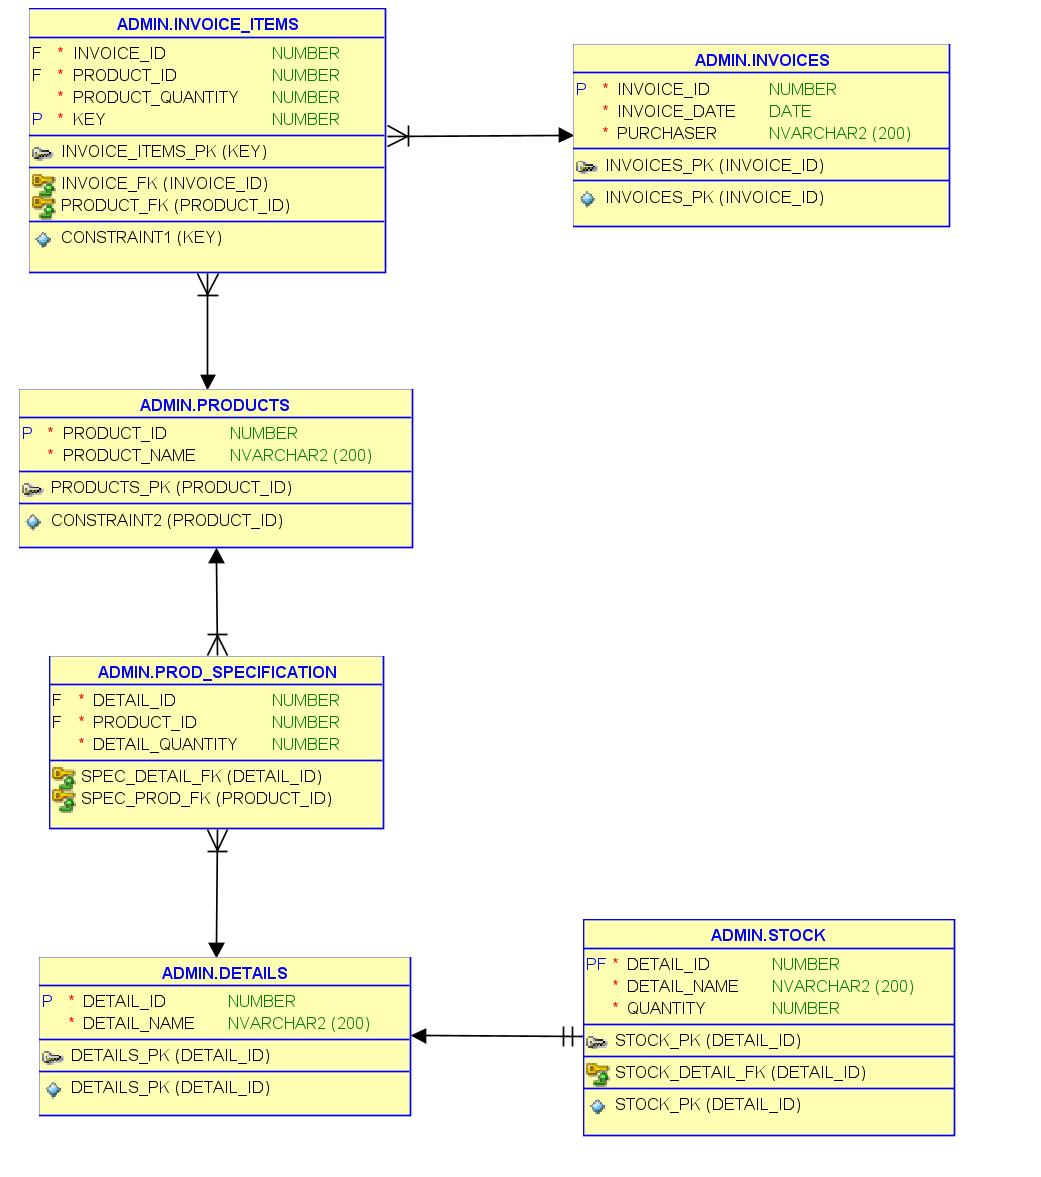
\includegraphics[width=0.8\textwidth,frame]{diagram.png}
   \caption{Projekt koncepcyjny bazy danych}
\end{figure}
\subsection{Tabela produktów}
\begin{tabular}{|c|l|l|} \hline
   \multicolumn{3}{|c|}{Products}             \\ \hline
   PK & product\_id   & int NOT NULL          \\ \hline
      & product\_name & varchar(200) NOT NULL \\ \hline
\end{tabular} \\
\vspace{0.3cm} \\
Tabela przechowuje wszystkie produkty możliwe do zamówienia. Każdy produkt ma
swój unikalny ID.

\subsection{Tabela faktur}
\begin{tabular}{|c|l|l|} \hline
   \multicolumn{3}{|c|}{Invoices}             \\ \hline
   PK & invoice\_id   & int NOT NULL          \\ \hline
      & invoice\_date & varchar(200) NOT NULL \\
      & purchaser     & varchar(200) NOT NULL \\ \hline
\end{tabular} \\
\vspace{0.3cm} \\
Tabela zawiera informacje o tym, kiedy zostało złożone zamówienie.
Kolumna purchaser zawiera informacje o nazwie podmiotu, który złożył zamówienie
- może być to firma lub osoba fizyczna. Dodanie faktury do tabeli powoduje
dodanie produktów zamówionych w ramach tej faktury do tabeli Invoice\_Items.

\subsection{Tabela pozycji na fakturach}
\begin{tabular}{|c|l|l|} \hline
   \multicolumn{3}{|c|}{Invoice\_Items}  \\ \hline
   FK & invoice\_id       & int NOT NULL \\ \hline
   FK & product\_id       & int NOT NULL \\
      & product\_quantity & int NOT NULL \\
   PK & key               & int NOT NULL \\ \hline
\end{tabular} \\
\vspace{0.3cm} \\
Tabela zawiera informacje o tym, jakie produkty \textit{product\_id} i jaka ich
ilość \textit{product\_quantity} została zamówiona w ramach danej faktury \textit{invoice\_id}.
Ze względu na użytą technologię wymagane było dodanie klucza głównego do tej tabelii.
\subsection{Tabela części}
\begin{tabular}{|c|l|l|} \hline
   \multicolumn{3}{|c|}{Details}                    \\ \hline
   PK & detail\_id   & int NOT NULL UNIQUE          \\ \hline
      & detail\_name & varchar(200) NOT NULL UNIQUE \\ \hline
\end{tabular} \\
\vspace{0.3cm} \\
Tabela przechowuje wszytskie możliwe detale potrzebne w firmie.

\subsection{Tabela stanu magazynowego}
\begin{tabular}{|c|l|l|} \hline
   \multicolumn{3}{|c|}{Stock}                         \\ \hline
   PK,FK & detail\_id   & int NOT NULL UNIQUE          \\ \hline
         & detail\_name & varchar(200) NOT NULL UNIQUE \\
         & quantity     & int NOT NULL                 \\ \hline
\end{tabular} \\
\vspace{0.3cm} \\
Tabela zawiera informacje o stanie magazynowym. Jeśli dany detal detail\_id,
jest dostępny na magazynie, to istnieje on w tej tabeli wraz z liczbą dostępnych
elementów. Jeśli jego liczba została zredukowana do 0 poprzez produkcję, zostaje
on automatycznie usunięty z magazynu.
\newpage
\subsection{Tabela specyfikacji produktu}
\begin{tabular}{|c|l|l|} \hline
   \multicolumn{3}{|c|}{Prod\_Specification} \\ \hline
   PK,FK & detail\_id       & int NOT NULL   \\ \hline
   FK    & product\_id      & int NOT NULL   \\
         & detail\_quantity & int NOT NULL   \\ \hline
\end{tabular} \\
\vspace{0.3cm} \\
Tabela przechowuje detale potrzebne do stworzenia produktu. Jeśli produkt ma
więcej niż jedną część, to tabela zawiera więcej rzędów o takim samym product\_id.
\section{Relacje między tabelami}
\begin{enumerate}
   \item Tabela Invoice\_Items zawiera kolumnę invoice\_id z tabeli Invoices.
         Relacja między tabelami to 1:N, ponieważ jedna faktura z tabeli
         Invoices może mieć jeden lub więcej odnośników w tabeli Invoice\_Items.
   \item Tabela Invoice\_Items zawiera w sobie również kolumnę product\_id z
         tabeli Products. Relacja pomiędzy tymi tabelami to również relacja jeden do
         wielu, ponieważ w wielu fakturach produkty mogą się powtarzać. Zatem Tabela
         Invoice\_Items może zawierać jeden lub więcej odnośników do jednego wiersza w
         tabeli Products.
   \item Tabela Prod\_Specification zawiera w sobie kolumnę product\_id z tabeli
         Products. Tutaj również zastosowana jest relacja 1:N, ponieważ jeden
         produkt może mieć jeden lub więcej elementów.
   \item Dodatkowo tabela Prod\_Specification zawiera kolumnę detail\_id z
         tabeli Details. Relacja pomiędzy tymi tabelami to 1:N, ponieważ w
         specyfikacji produktów będzie wielokrotnie występował dany element.
   \item Tabela Stock zawiera kolumnę detail\_id z tabeli Details. Relacja
         pomiędzy tymi tabelami to jeden do jednego, ponieważ jeden wiersz w tabeli
         stock będzie odpowiadał jednemu wierszowi z tabeli Details.
\end{enumerate}

\section{Funkcjonalności oraz prawa dostępu poszczególnych grup użytkowników}
\begin{enumerate}
   \item Grupa Zamawiających
         \begin{itemize}
            \item Wgląd w listę dostępnych produktów.
            \item Składanie zamówienia na dane produkty.
         \end{itemize}
   \item Grupa administratorów
         \begin{itemize}
            \item Wgląd w listę dostępnych produktów.
            \item Podgląd stanów magazynowych.
            \item Podgląd złożonych zamówień.
            \item Automatyczne zamawianie części do magazynu, jeśli w złożonym
                  zamówieniu są produkty, do których brakuje elementów.
            \item Podgląd specyfikacji produktów.
         \end{itemize}
   \item Inne funkcjonalności:
         \begin{itemize}
            \item Stany magazynowe są automatycznie aktualizowane po złożeniu
                  zamówienia przez Zamawiającego.
            \item Automatyczne zamawianie części do magazynu, jeśli w złożonym
                  zamówieniu są produkty, do których brakuje elementów.
         \end{itemize}
\end{enumerate}
\newpage
\section{Początek prac nad aplikacją}
\paragraph{}
Pracę nad aplikacją rozpoczeliśmy od przemyślenia funkcjonalności aplikacji.
Nastęnie przeszliśmy do zaprojektowania tabel i połączeń między
nimi, co zostało zaprezentowane w punktach 3 oraz 4. Kolejnym krokiem było
zapoznanie się z narzędziem pracy od firmy Oracle oraz składnią języka SQL.
\subsection{Tworzenie bazy danych oraz tabel}
Stworzenie bazy danych odbywa się poprzez wydanie komendy \textit{CREATE
   DATABASE nazwa\_bazy\_danych}. Tworzenie tabel w języku SQL odbywa się poprzez korzystanie z komendy
\textit{CREATE TABLE nazwa\_tabeli}. Poszczególne kolumny tabeli wymiania się po
otworzeniu nawiasów. Należy określić rodzaj danych w poszczególnych kolumnach
oraz klucze tabeli. Dodatkowo można określić ograniczenia dla poszczególnych
kolumn tabeli.

Poniżej znajdują się komendy potrzebne do stworzenia poszczególnych tabel
wraz z komendami użytymi do stworzenia wyzwalaczy ustawiających klucz
główny każdego kolejego rzędu o jeden większy od poprzedniego. Zostały do
tego użyte sekwencje zaprezentowane w kolejnym punkcie.
\subsubsection{Tworzenie tabeli faktur}
\begin{lstlisting}[language=SQL,frame=single]
  CREATE TABLE INVOICES 
   (	INVOICE_ID NUMBER NOT NULL , 
	INVOICE_DATE DATE NOT NULL , 
	PURCHASER NVARCHAR2(200) NOT NULL , 
	 CONSTRAINT INVOICES_PK PRIMARY KEY (INVOICE_ID)
   ) 
\end{lstlisting}
\begin{lstlisting}[language=SQL,frame=single]
  CREATE OR REPLACE TRIGGER INVOICES_TRIGGER1 
BEFORE INSERT ON INVOICES
FOR EACH ROW
BEGIN
	SELECT INVOICE_ID_SEQUENCE.NEXTVAL
	INTO :NEW.INVOICE_ID
	FROM DUAL;
END;
/
\end{lstlisting}

\subsubsection{Tworzenie tabeli produktów zamówionych w ramach faktur}
\begin{lstlisting}[language=SQL,frame=single]
  CREATE TABLE INVOICE_ITEMS 
   (	INVOICE_ID NUMBER NOT NULL , 
	PRODUCT_ID NUMBER NOT NULL , 
	PRODUCT_QUANTITY NUMBER NOT NULL , 
	KEY NUMBER NOT NULL , 
	 CONSTRAINT INVOICE_ITEMS_PK PRIMARY KEY (KEY),
	 CONSTRAINT INVOICE_FK FOREIGN KEY (INVOICE_ID)
	  REFERENCES INVOICES (INVOICE_ID) , 
	 CONSTRAINT PRODUCT_FK FOREIGN KEY (PRODUCT_ID)
	  REFERENCES PRODUCTS (PRODUCT_ID) 
   )
\end{lstlisting}
\newpage
\begin{lstlisting}[language=SQL,frame=single]
  CREATE OR REPLACE TRIGGER INVOICE_ITEMS_TRIGGER1 
BEFORE INSERT ON INVOICE_ITEMS
FOR EACH ROW
BEGIN
	SELECT INVOICE_ITEM_SEQUENCE.NEXTVAL
	INTO :NEW.KEY
	FROM DUAL;
END;
/
\end{lstlisting}

\subsubsection{Tworzenie tabeli produktów}
\begin{lstlisting}[language=SQL,frame=single]
  CREATE TABLE PRODUCTS 
   (	PRODUCT_ID NUMBER NOT NULL , 
	PRODUCT_NAME NVARCHAR2(200) NOT NULL , 
	 CONSTRAINT PRODUCTS_PK PRIMARY KEY (PRODUCT_ID)
   )
\end{lstlisting}
\begin{lstlisting}[language=SQL,frame=single]
  CREATE OR REPLACETRIGGER PRODUCTS_TRIGGER1 
BEFORE INSERT ON PRODUCTS
FOR EACH ROW
BEGIN
	SELECT PRODUCT_ID_SEQUENCE.NEXTVAL
	INTO :NEW.PRODUCT_ID
	FROM DUAL;
END;
/
\end{lstlisting}

\subsubsection{Tworzenie tabeli części}
\begin{lstlisting}[language=SQL,frame=single]
   CREATE TABLE DETAILS 
   (	DETAIL_ID NUMBER NOT NULL , 
	DETAIL_NAME NVARCHAR2(200) NOT NULL , 
	 CONSTRAINT DETAILS_PK PRIMARY KEY (DETAIL_ID)
   )
\end{lstlisting}
\begin{lstlisting}[language=SQL,frame=single]
  CREATE OR REPLACE TRIGGER DETAILS_TRIGGER1 
  BEFORE INSERT ON DETAILS
FOR EACH ROW
BEGIN
	SELECT DETAIL_ID_SEQUENCE.NEXTVAL
	INTO :NEW.DETAIL_ID
	FROM DUAL;
END;
/
\end{lstlisting}

\newpage
\subsubsection{Tworzenie tabeli specyfikacji produktów}
\begin{lstlisting}[language=SQL,frame=single]
  CREATE TABLE PROD_SPECIFICATION 
   (	DETAIL_ID NUMBER NOT NULL , 
	PRODUCT_ID NUMBER NOT NULL , 
	DETAIL_QUANTITY NUMBER NOT NULL , 
	 CONSTRAINT SPEC_PROD_FK FOREIGN KEY (PRODUCT_ID)
	  REFERENCES PRODUCTS (PRODUCT_ID) , 
	 CONSTRAINT SPEC_DETAIL_FK FOREIGN KEY (DETAIL_ID)
	  REFERENCES DETAILS (DETAIL_ID) 
   ) 
\end{lstlisting}

\subsubsection{Tworzenie tabeli magazynu}
\begin{lstlisting}[language=SQL,frame=single]
  CREATE TABLE STOCK 
   (	DETAIL_ID NUMBER NOT NULL , 
	DETAIL_NAME NVARCHAR2(200) NOT NULL , 
	QUANTITY NUMBER NOT NULL , 
	 CONSTRAINT STOCK_PK PRIMARY KEY (DETAIL_ID), 
	 CONSTRAINT STOCK_DETAIL_FK FOREIGN KEY (DETAIL_ID)
	  REFERENCES DETAILS (DETAIL_ID)
\end{lstlisting}

\subsection{Tworzenie sekwencji}

Użycie sekwencji zapewnia nam unikalność klucza głównego, który będzie zaczynał
się od wartości 1 i zwiększał się z każdym kolejnym rzędem o 1. Stworzyliśmy 4
sekwencje, które zostały użyte w wyzwalaczach w poszczególnych tabelach.

\begin{lstlisting}[language=SQL,frame=single]
   CREATE SEQUENCE  DETAIL_ID_SEQUENCE 
   START WITH 1
   INCREMENT BY 1
   NOCACHE
   NOCYCLE;
 \end{lstlisting}

\subsection{Dodawanie danych do tabeli}
Dodawanie danych do tabeli odbywa się poprzez korzystanie z komendy
\textit{INSERT INTO nazwa\_tabeli (kolumna1, kolumna2) VALUES
   (wartość1, wartość2)}. Komenda ta nie musi zawierać wypisanych nazw kolumn, pod
warunkiem, że wpychamy do tabeli całe wiersze danych.
Poniżej przedstawione jest przykładowe dodanie produktu do tabeli Products.

\begin{lstlisting}[language=SQL,frame=single]
INSERT INTO Products (product_name) VALUES ('odkurzacz');
 \end{lstlisting}

\section{Implementacja}
\paragraph{}
Pracę nad implementacją rozpoczęliśmy od połączenia aplikacji z naszą bazą danych.
Skorzystaliśmy z mapowania bazy danych do przestrzeni obiektowej za pomocą Entity Framework, by móc odnosić
się do poszczególnych elementów z pozycji programu.
W kolejnym kroku zaczęliśmy pracę nad implementowaniem założonych funkcjonalności systemu.
Rozpoczęliśmy od możliwości zamawiania produktów, ponieważ potrzebna ona była do pozostałych
funkcjonalności. Początkowo system zamawiania polegał na wybraniu produktu z rozwijanej listy i
wpisaniu ilości produktu, jaką chcemy zamówić. Okno wpisywania zostało zabezpieczone zgodnie z
zasadami walidacji danych.
Następnym krokiem było utworzenie strony wyświetlającej potwierdzenie zamówienia oraz strony
wyświetlającej części potrzebne do produkcji danego przedmiotu. W tym kroku stworzyliśmy również
podział na widoki: widok administratora oraz widok zwykłego użytkownika. Strona wyświetlająca części
zamienne została przypisana do widoku administratora, zaś strona z potwierdzeniem została przypisana do
widoku zwykłego użytkownika. Następnie dodaliśmy przeglądanie części znajdujących się w magazynie
oraz dodaliśmy możliwość przeglądania zamówień, realizacji zamówień oraz kasowania zamówień.
W kolejnym kroku zaimplementowaliśmy widok logowania do panelu administratora. Do panelu administratora
dodaliśmy również możliwość ręcznego zamawiania części do magazynu. Administrator uzyskał również
możliwość podglądu szczegółów dotyczących faktur oraz części potrzebnych do konkretnego zamówienia.
Po pierwszych testach wprowadziliśmy zmiany w panelu użytkownika. Zamiast zamawiania produktów z
rozwijanej listy wprowadziliśmy przeglądanie produktów kolejnymi stronami. Do produktów dodaliśmy
zdjęcia oraz przycisk dodawania do koszyka wraz z konkretną ilością. W pasku nawigacyjnym
umieściliśmy koszyk. Zaimplementowaliśmy dla niego osobną stronę prezentującą zawartość koszyka oraz
zajmującą się ostatecznym składaniem zamówienia. Po konsulatcji, wprowadziliśmy dodatkową tabelę w
bazie danych. Tabela służy do przechowywania historii zamówień.
Poniżej przedstawiona jest ostateczna struktura bazy danych znajdującej się w naszym projekcie.
\begin{figure}[H]
   \centering
   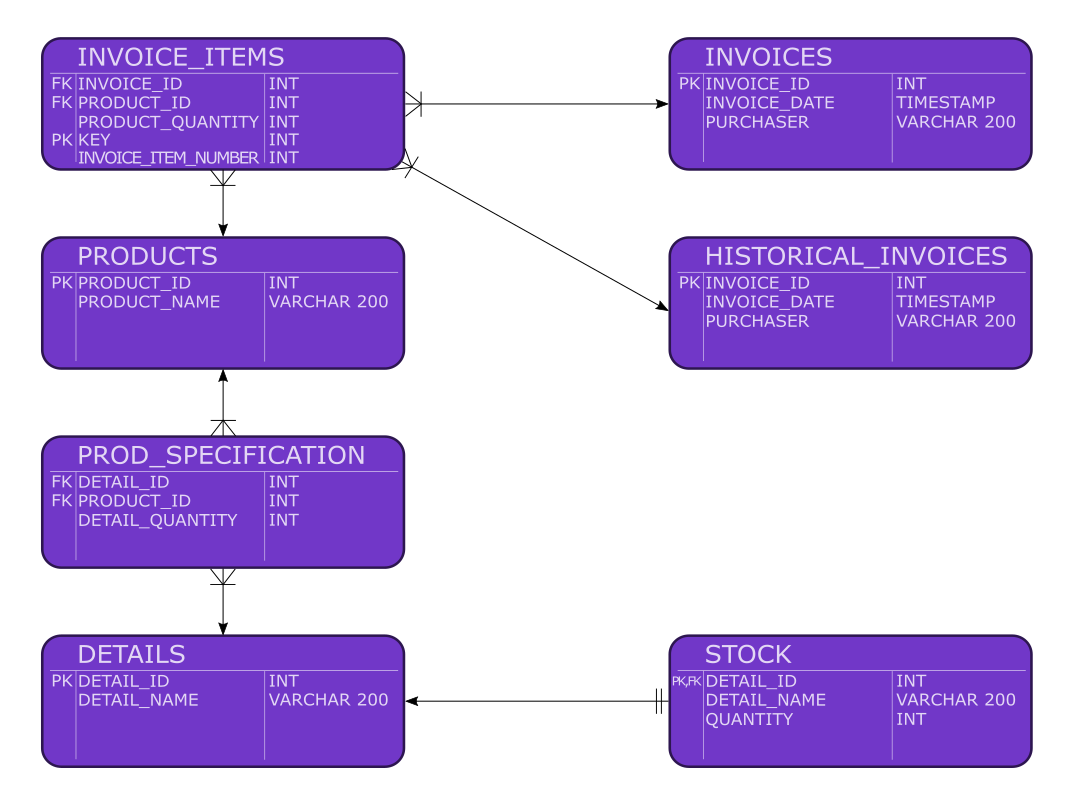
\includegraphics[width=0.8\textwidth,frame]{diagram_f.png}
   \caption{Struktura bazy danych}
\end{figure}
\begin{figure}[H]
   \centering
   \begin{tabular}{|c|l|l|} \hline
      \multicolumn{3}{|c|}{Historical\_Invoices} \\ \hline
      PK & invoice\_id   & int NOT NULL          \\ \hline
         & invoice\_date & varchar(200) NOT NULL \\
         & purchaser     & varchar(200) NOT NULL \\ \hline
   \end{tabular} \\
\end{figure}
\vspace{0.3cm}
Tabela zawiera informacje o tym, kiedy było złożone zamówienie.
Kolumna purchaser zawiera informacje o nazwie podmiotu, który złożył zamówienie
- może być to firma lub osoba fizyczna. Kolumna z numerem id faktury (invoice\_id) pozwoliła nam na
dostanie informacji o szczegółach historycznego zamówienia potrzebnych do implementacji funkcji
automatycznego zamawiania na podstawie historii z ostatniego miesiąca. Oprócz dodania tabeli
historycznej dodaliśmy również kolumnę w tabeli ``Invoice\_Items''. Służy ona do przypisania pozycji
produktu na fakturze. Kolejnym krokiem była implementacja systemu automatycznego zamawiania. Funkcja ta jest oparta na przeszukiwaniu tabeli
historycznej w celu uzyskania zamówień z ostatniego miesiąca oraz na ustawieniu odpowiedniej komendy
w programie Cron. Służy on do ustalania harmonogramu wykonywania danych zadań, przykładowo do
co tygodniowego wykonania uzupełnienia magazynu. Ostatnim krokiem w implementacji projektu była
implementacja zabezpieczeń bazy danych przed jednoczesnym zapisem użytkowników do tabel.
Zabezpieczenie jest o tyle istotne, ponieważ zakładamy w naszym projekcie wielu administratorów/
realizatorów zamówień.

\section{Testowanie}
\paragraph{}
Aby przetestować działanie aplikacji wprowadziliśmy testy jednostkowe do poszczególnych funkcji w
programie.
Najistotniesze działanie mają funkcje pobierające dane od użytkownika i przekształcające je do
odpowiedniego formatu, a nastepnie przekazujące dane do zapisu do bazy danych.

\section{Prezentacja ostatecznego wyglądu aplikacji}
\subsection{Widok zwykłego użytkownika}

\subsubsection{Strona główna}
\begin{figure}[H]
   \centering
   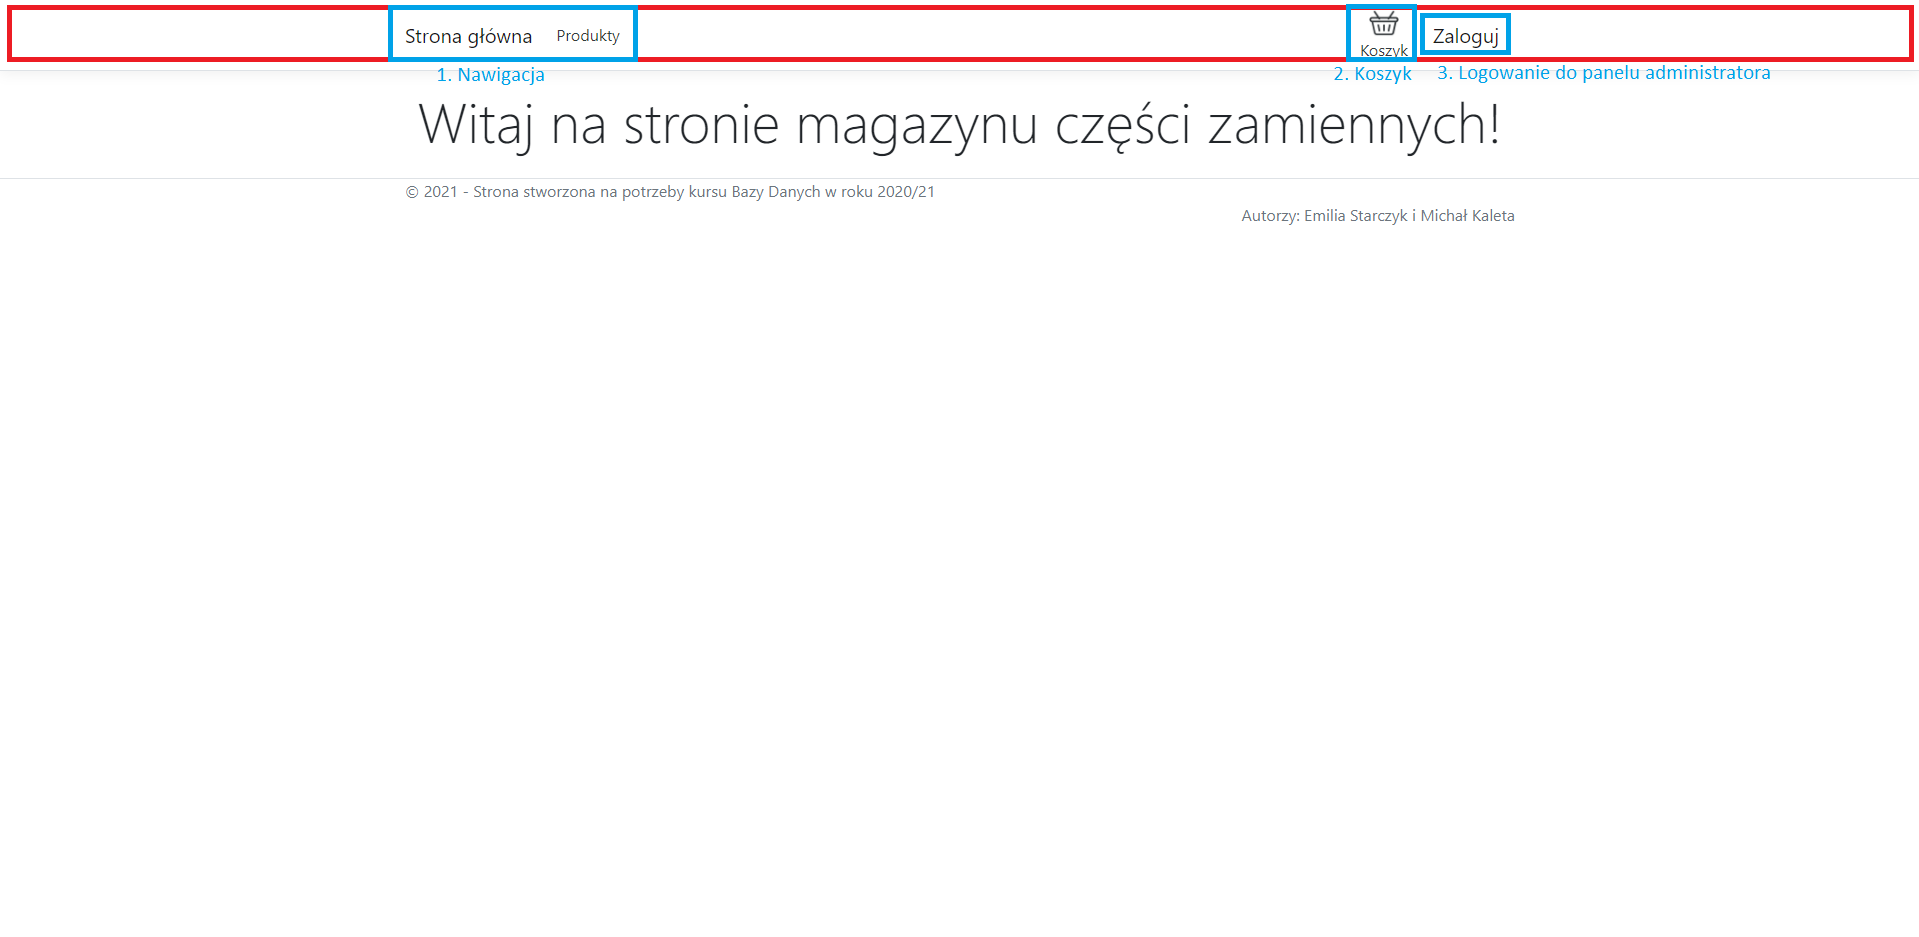
\includegraphics[width=0.99\textwidth,frame]{Wyglad/powitanie_uzytkownik.png}
   \caption{Strona główna - strona powitania}
\end{figure}
Strona główna przedstawia widok, jaki widzimy zaraz po wejściu na stronę www naszego projektu.
Na stronie widnieje powitanie. Poruszanie się po stronie zapewnione jest przez nas za pomocą paska
nawigacyjnego. Numerem jeden w niebieskiej obramówce oznaczone jest miejsce nawigacji pomiędzy
poszczególnymi stronami. Pod numerem dwa znajduje się przycisk przejścia do strony z koszykiem.
Numer 3 jest przyciskiem logowania do panelu administratora.
\subsubsection{Produkty}
\begin{figure}[H]
   \centering
   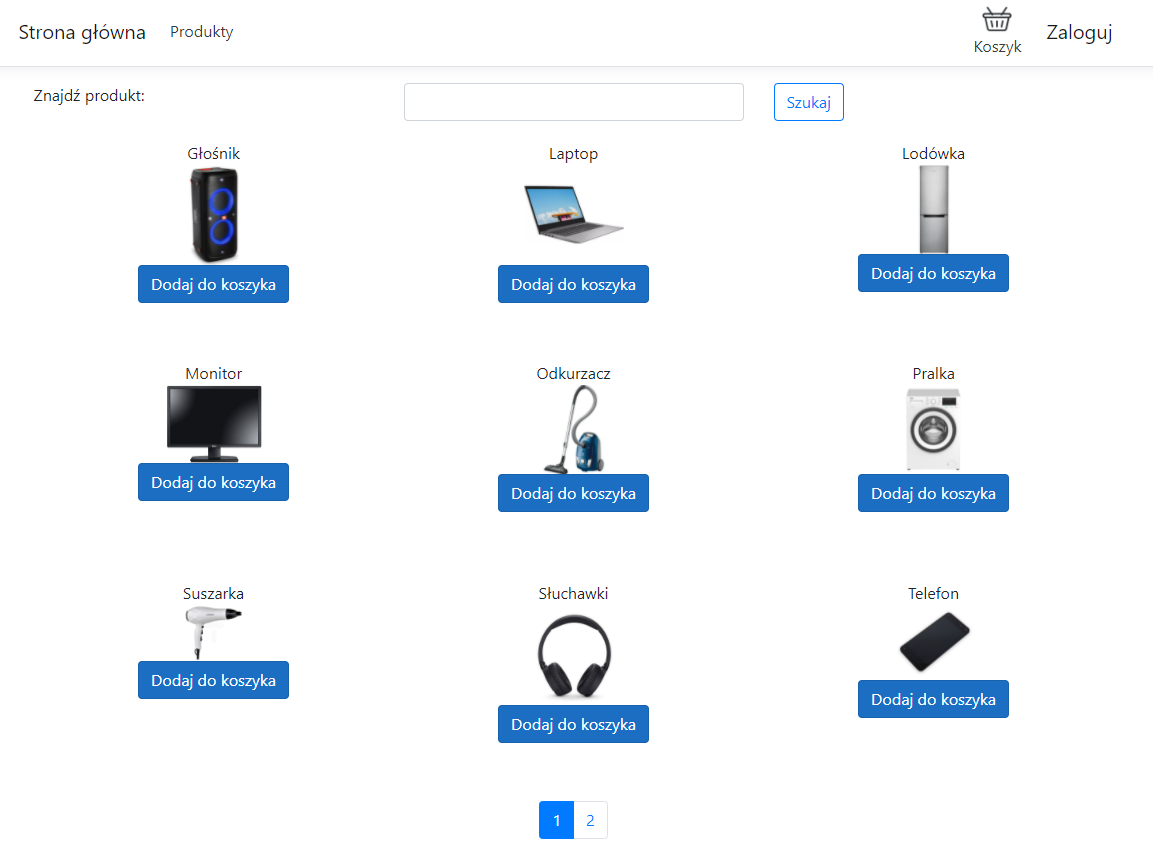
\includegraphics[width=0.7\textwidth,frame]{Wyglad/produkty.png}
   \caption{Przegląd dostępnych produktów}
\end{figure}
\begin{figure}[h]
   \centering
   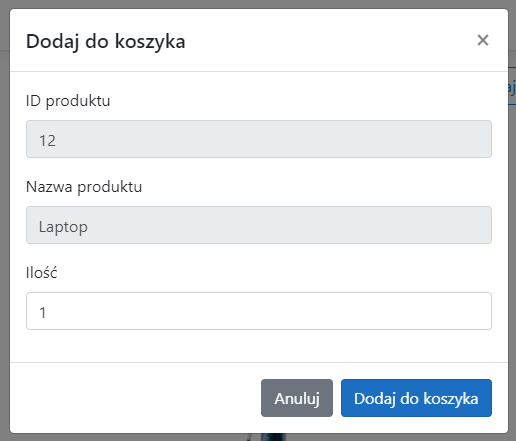
\includegraphics[width=0.4\textwidth,frame]{Wyglad/dodaj_koszyk.png}
   \caption{Okno dodawania produktu do koszyka}
\end{figure}
Strona pozwalająca na przeglądanie produktów dostępnych do zakupu stanowi
kluczową część naszego projektu. Potencjalni klienci mogą oglądać jakie produkty
są dostępne do zamówienia oraz dodać je do koszyka z tego samego miejsca.
Dodawanie do koszyka odbywa się na tej samej stronie, za pomocą okna modalnego,
w którym możemy wybrać ilość produktów którą chcemy dodać do koszyka.

\subsubsection{Koszyk}
\begin{figure}[H]
   \centering
   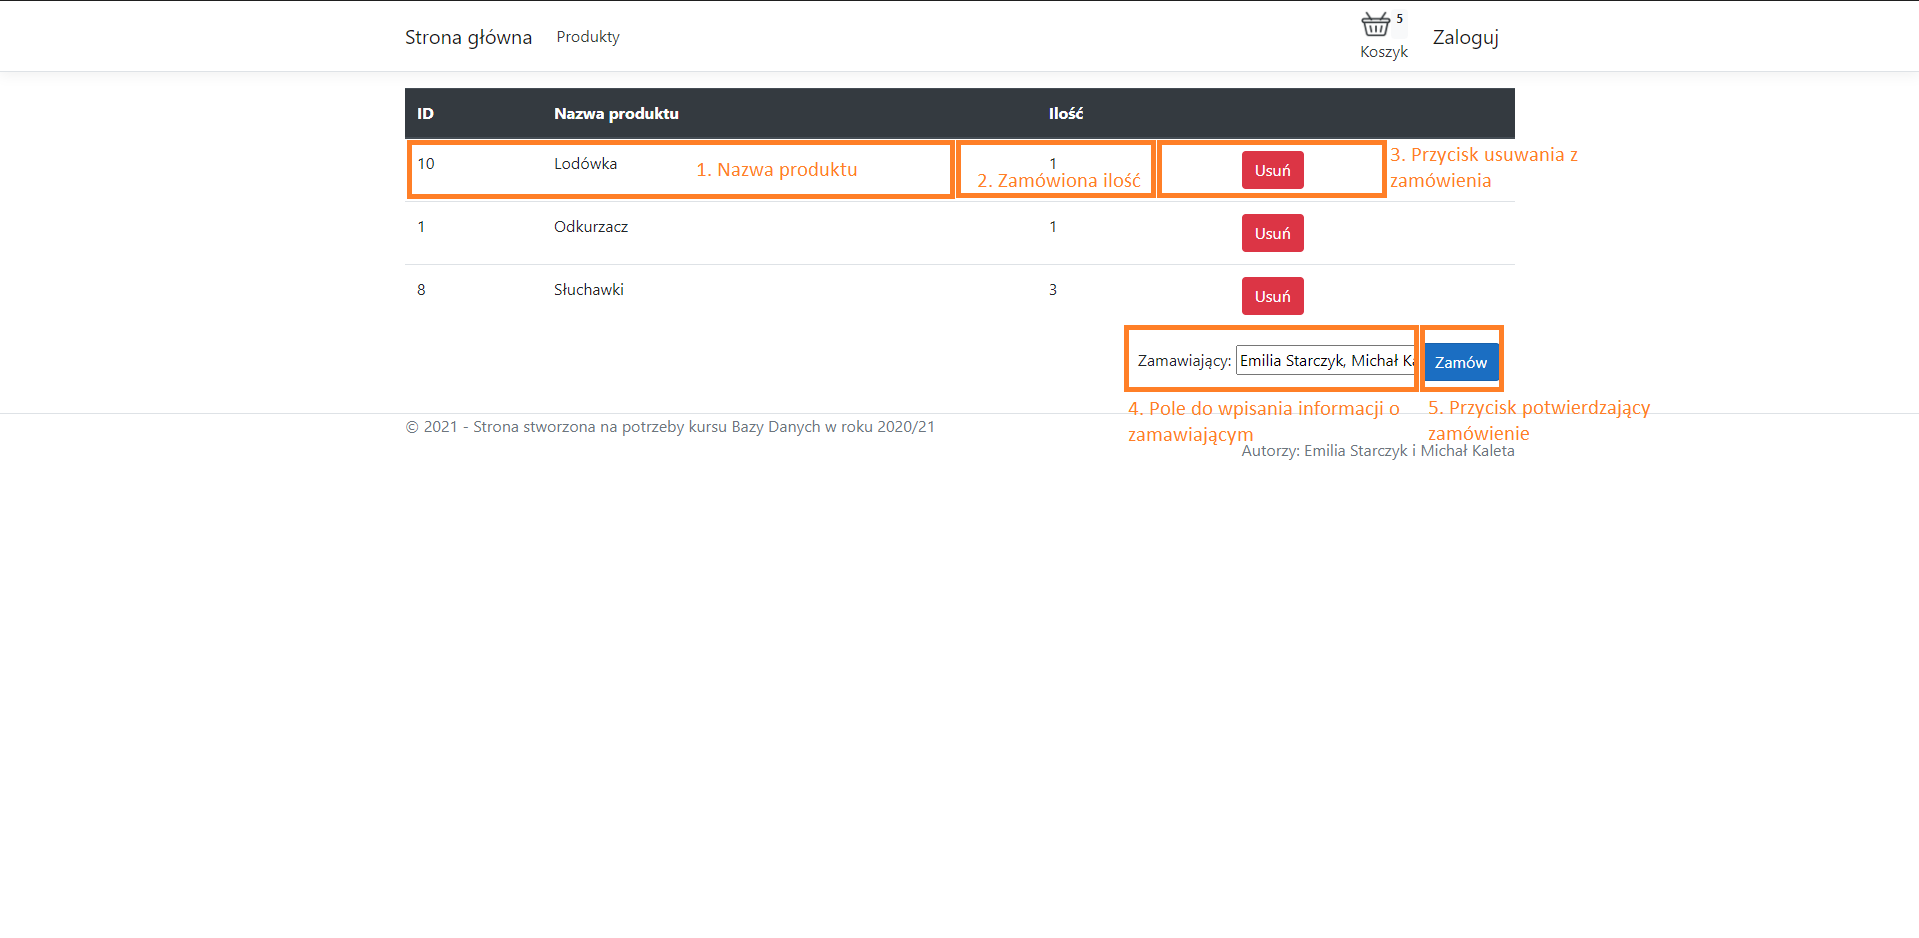
\includegraphics[width=0.99\textwidth,frame]{Wyglad/koszyk_uzytkownik.png}
   \caption{Koszyk}
\end{figure}
Powyższe zdjęcie przedstawia stronę z zawartością koszyka. Składa się ona z kilku elemenetów:
\begin{enumerate}
   \item Nazwa produktu - nazwa zamówionego przez użytkownika produktu.
   \item Pole z zamówioną ilością.
   \item Przycisk do usuwania produktu z zamówienia.
   \item Pole Zamawiający - pole do wpisania informacji o zamawiającym.
   \item Przycisk zamów - przycisk potwierdzenia zamówienia. Po wciśnięciu tego przycisku następuje
         przejście do strony potwierdzenia z informacją o zamówionych produktach.
\end{enumerate}

\subsubsection{Potwierdzenie zamówienia}
\begin{figure}[H]
   \centering
   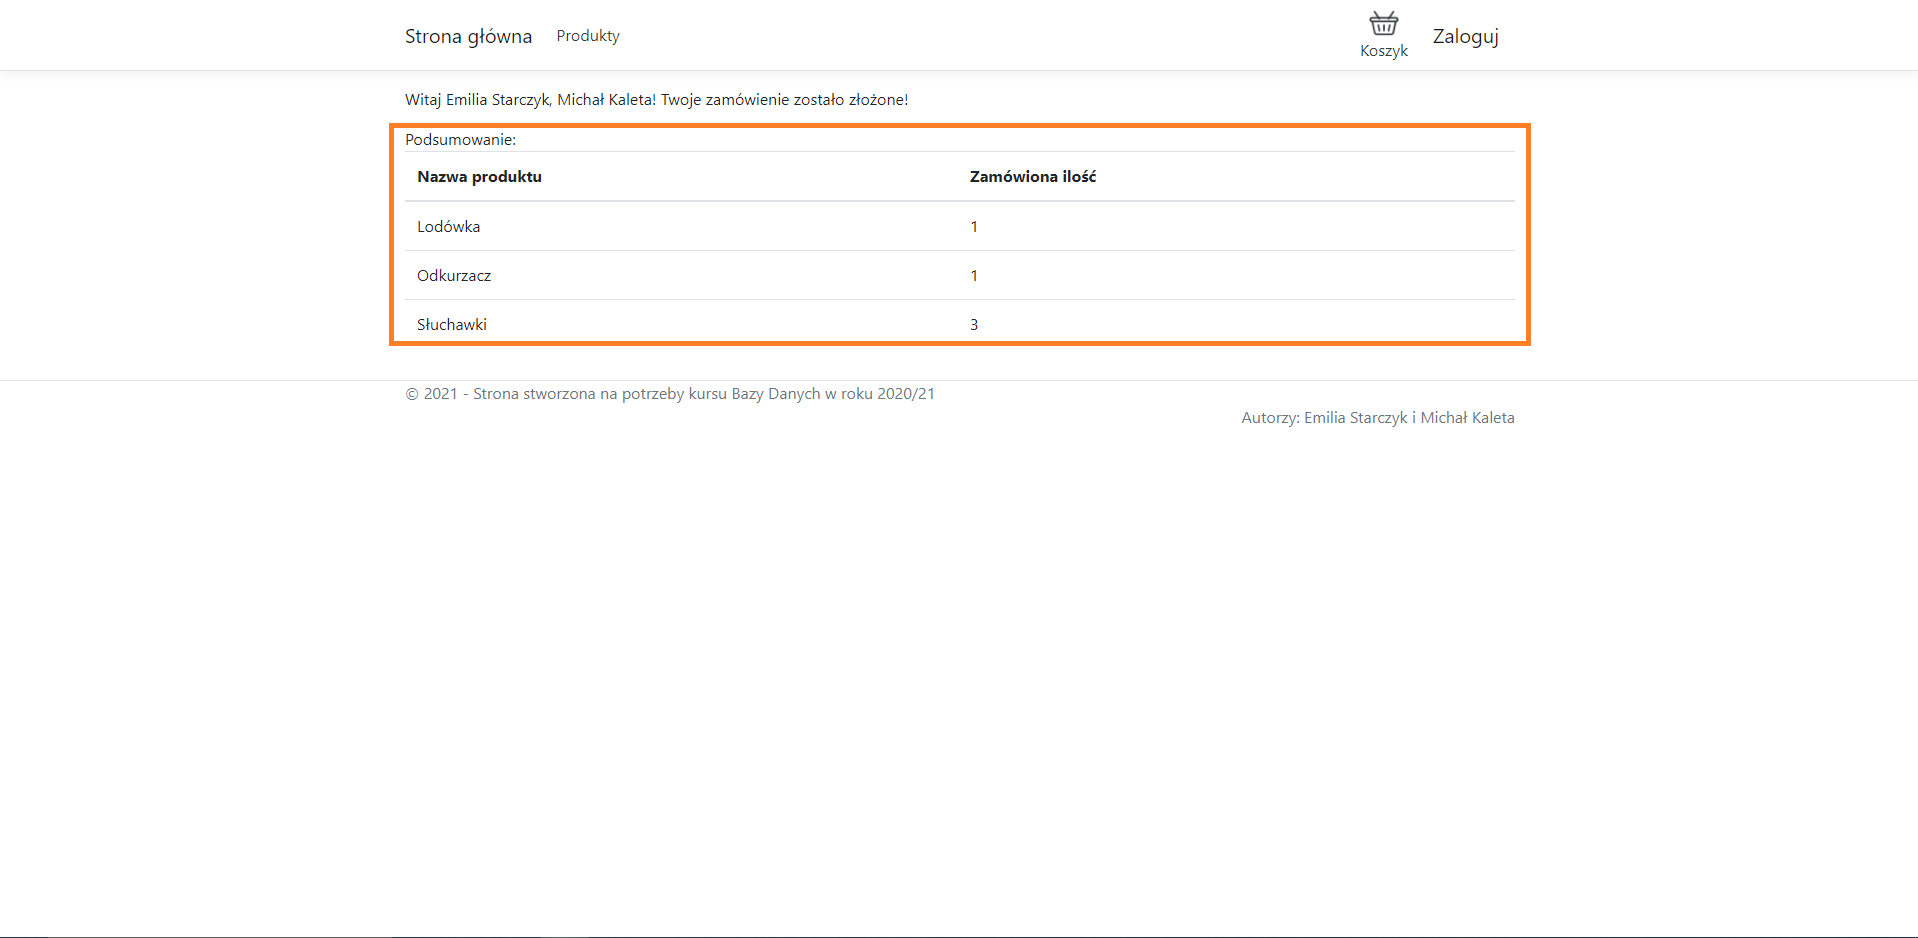
\includegraphics[width=0.99\textwidth,frame]{Wyglad/zlozenie_zamowienia_uzytkownik.png}
   \caption{Strona zawierająca potwierdzenie zamówienia}
\end{figure}
Na powyższym zdjęciu przedstawiona jest zawartość strony potwierdzającej zamówienie produktów. W
pomarańczowej ramce przedstawiona jest lista zamówionych produktów.

\subsection{Widok administratora}
\subsubsection{Zaloguj}
\begin{figure}[H]
   \centering
   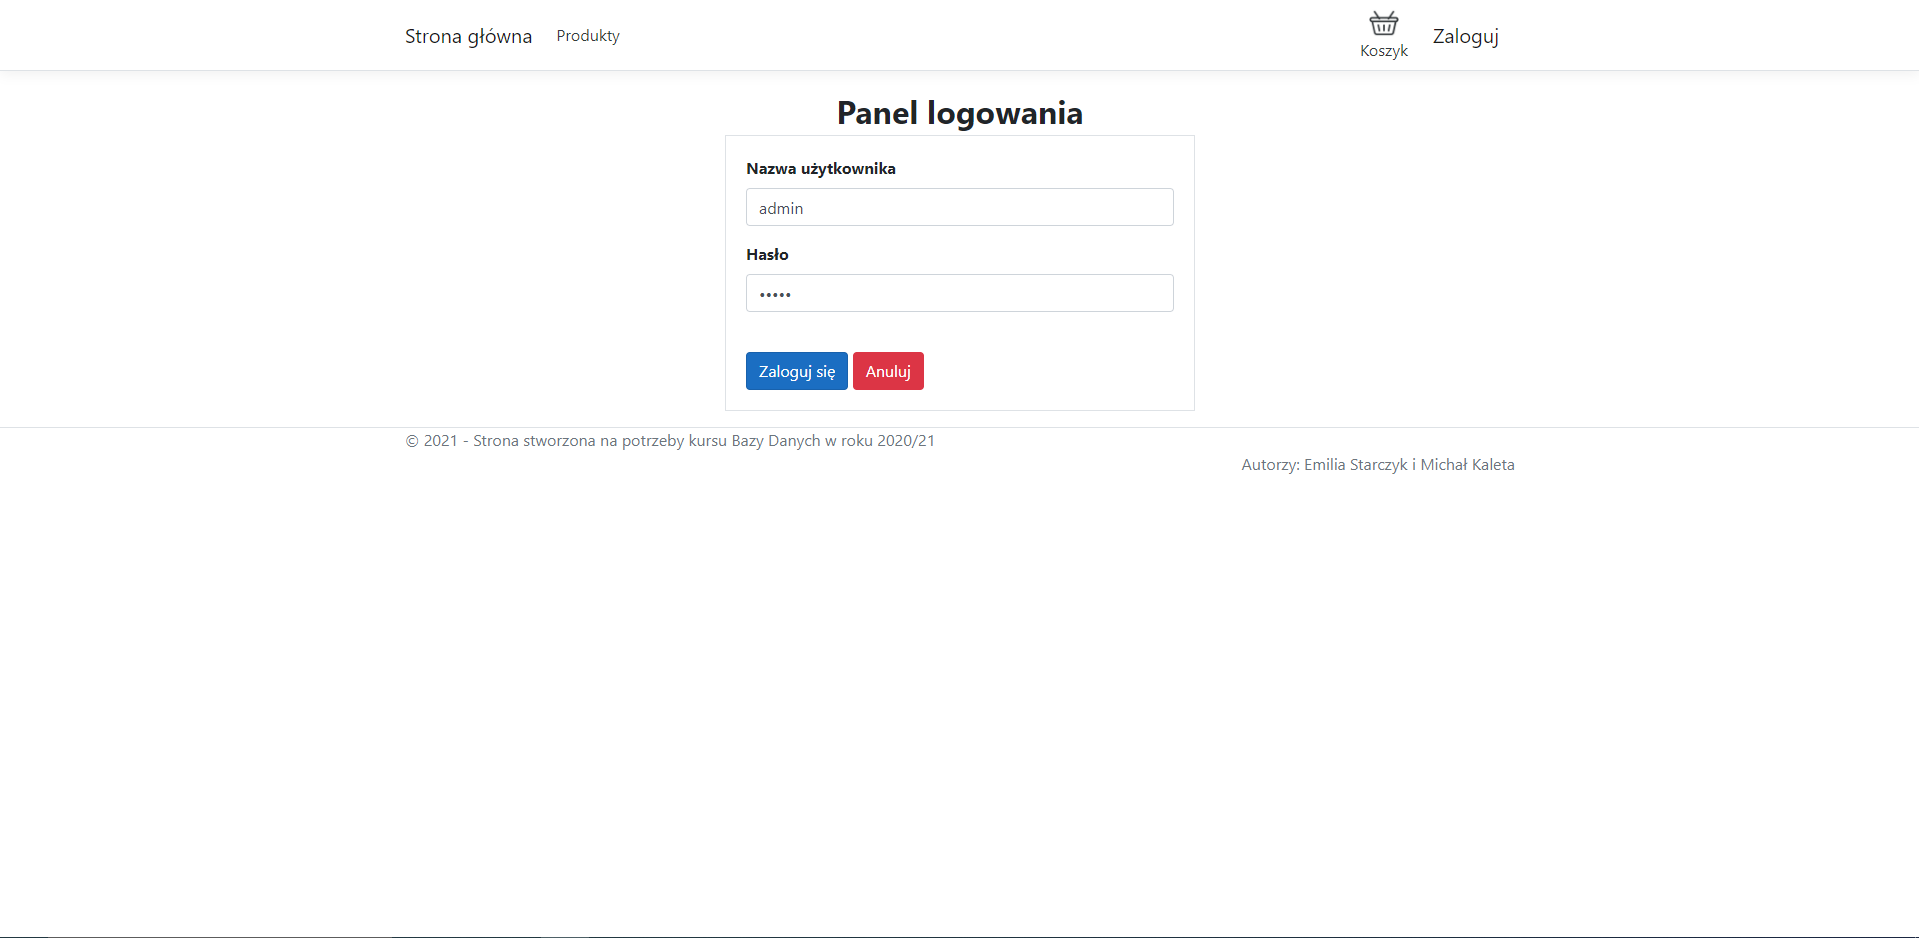
\includegraphics[width=0.99\textwidth,frame]{Wyglad/logowanie_admin.png}
   \caption{Panel logowania do widoku administratora}
\end{figure}
W miejsce ``Nazwa użytkownika'' oraz ``Hasło'' administrator musi podać prawidłowe dane. Po uzupełnieniu
danych i naciśnięciu przycisku ``Zaloguj się'' następuje przekierowanie do pełnego widoku administratora.

\subsubsection{Strona główna}
\begin{figure}[H]
   \centering
   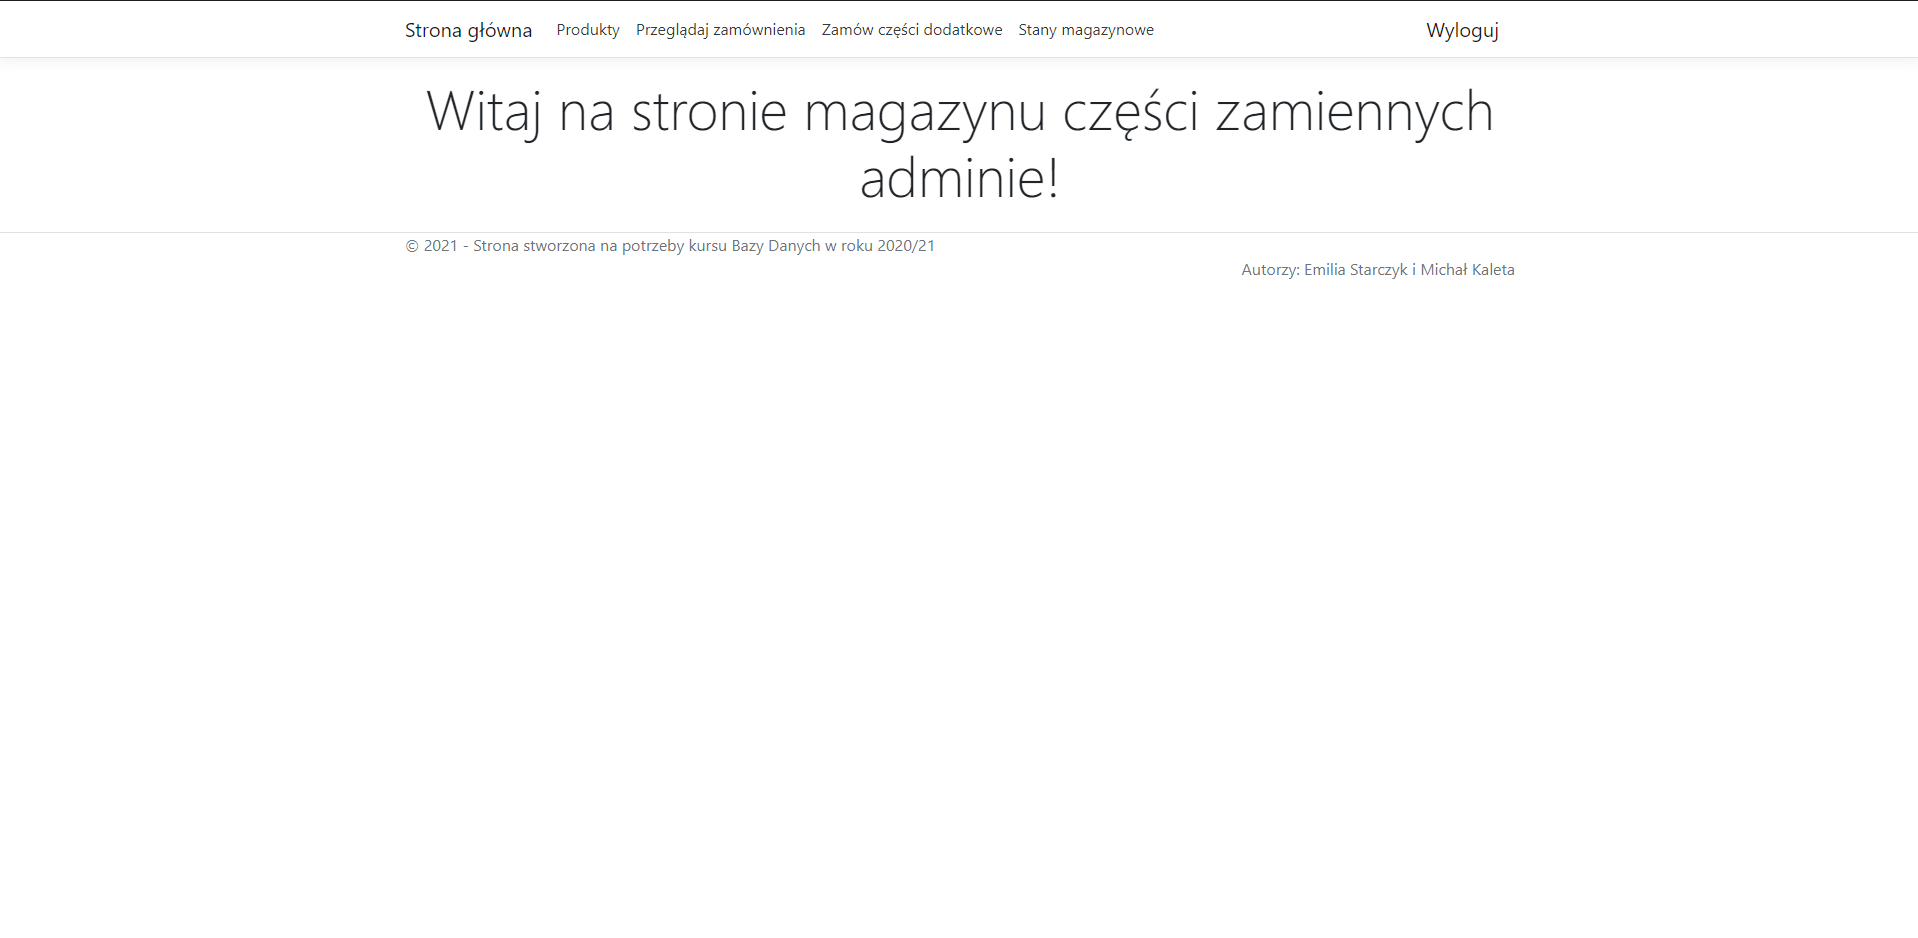
\includegraphics[width=0.99\textwidth,frame]{Wyglad/powitanie_admin.png}
   \caption{Strona główna widoku administratora}
\end{figure}
Widok ten zostaje wyświetlony tuż po zalogowaniu. Jest to widok rozszerzony w stosunku do widoku
zwykłego użytkownika. Poruszanie się również zapewnione jest poprzez pasek nawigacyjny. Dodatkowe
funkcje/widoki, przyznane administratorowi opisane będą w następnych punktach.

\subsubsection{Produkty}
\begin{figure}[H]
   \centering
   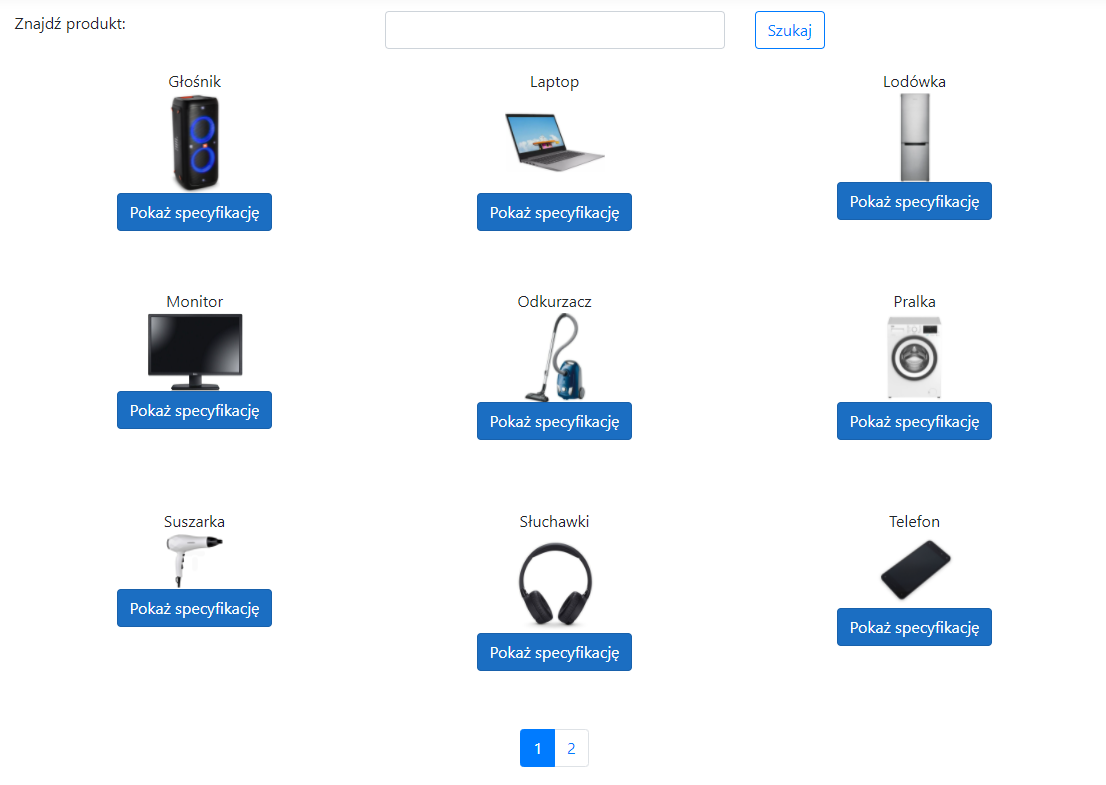
\includegraphics[width=0.8\textwidth,frame]{Wyglad/produkty_admin.png}
   \caption{Widok strony podglądu produktów w układzie administratora}
\end{figure}
Strona wyświetlająca produkty w widoku administrora jest bardzo podobna do
zwykłego podglądu - różnicą jest przycisk znajdujący się pod każdym produktem,
który w przypadku administratora przekieruje nas na stronę specyfikacji
produktu.

\subsubsection{Specyfikacja produktu}
\begin{figure}[H]
   \centering
   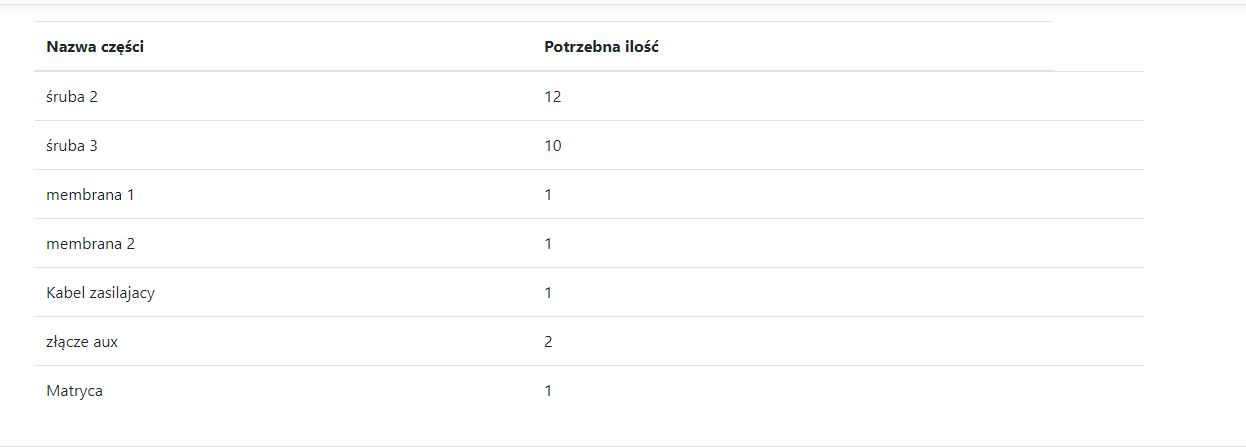
\includegraphics[width=0.8\textwidth,frame]{Wyglad/spec.png}
   \caption{Podgląd specyfikacji pojedynczego produktu}
\end{figure}
Strona wyświetlająca specyfikację produktu pozwala sprawdzić jakie części są
wymagane dla danego produktu.

\subsubsection{Przeglądaj zamówienia}
\begin{figure}[H]
   \centering
   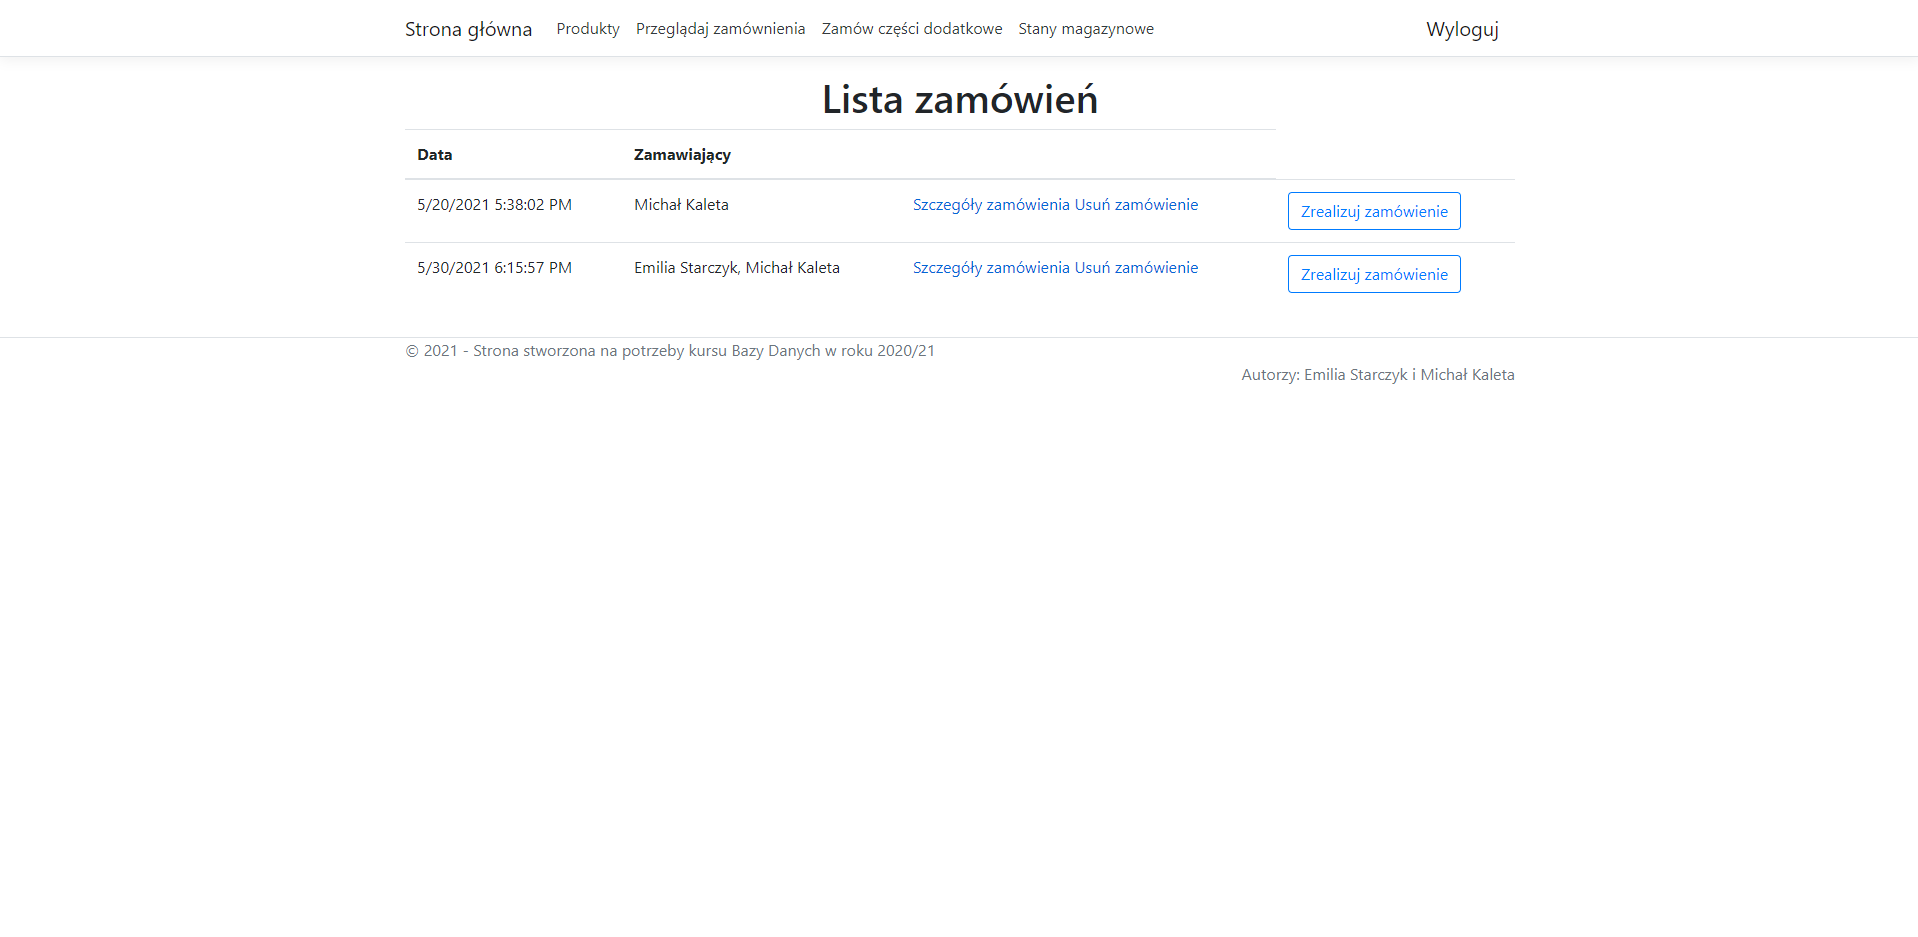
\includegraphics[width=0.99\textwidth,frame]{Wyglad/lista_zamowien_admin.png}
   \caption{Strona zapewniająca podgląd listy złożonych zamówień}
\end{figure}
Widok tej strony pojawia się po wciśnięciu odpowiedniego przycisku w pasku nawigacyjnym.
Administrator ma tutaj dostęp do listy złożonych zamówień. Oprócz tego może podejrzeć szczegóły
każdego zamówienia naciskając przycisk ``Szczegóły zamówienia''. Dodatkowo wyposażyliśmy
administratora w możliwość usuwania złożonego zamówienia oraz możliwość realizacji zamówienia.
Naciskając niebieski tekst ``Usuń zamówienie'' spowodujemy usunięcie konkretnego zamówienia z bazy
danych. Naciśnięcie przycisku ``Zrealizuj zamówienie'' powoduje wywołanie
procedury sprawdzającej wymagany stan magazynowy, i w przypadku wystarczających
ilości są one usuwane z magazynu a samo zamówienie jest przenoszone do tabeli
zamówień historycznych.

\begin{itemize}
   \item Panel ``Szczegóły zamówienia''\\
         \newline
         \fbox{
            \parbox[c]{0.92\textwidth}{
               \centering
               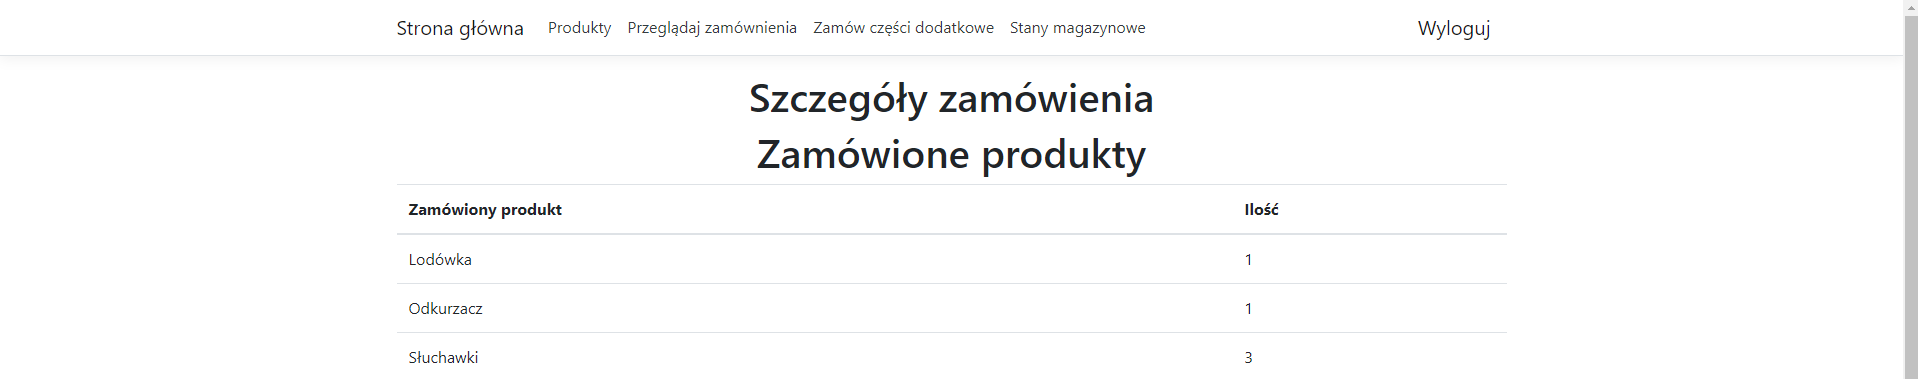
\includegraphics[width=0.6\textwidth]{Wyglad/szczegoly_zam1_admin.png}
               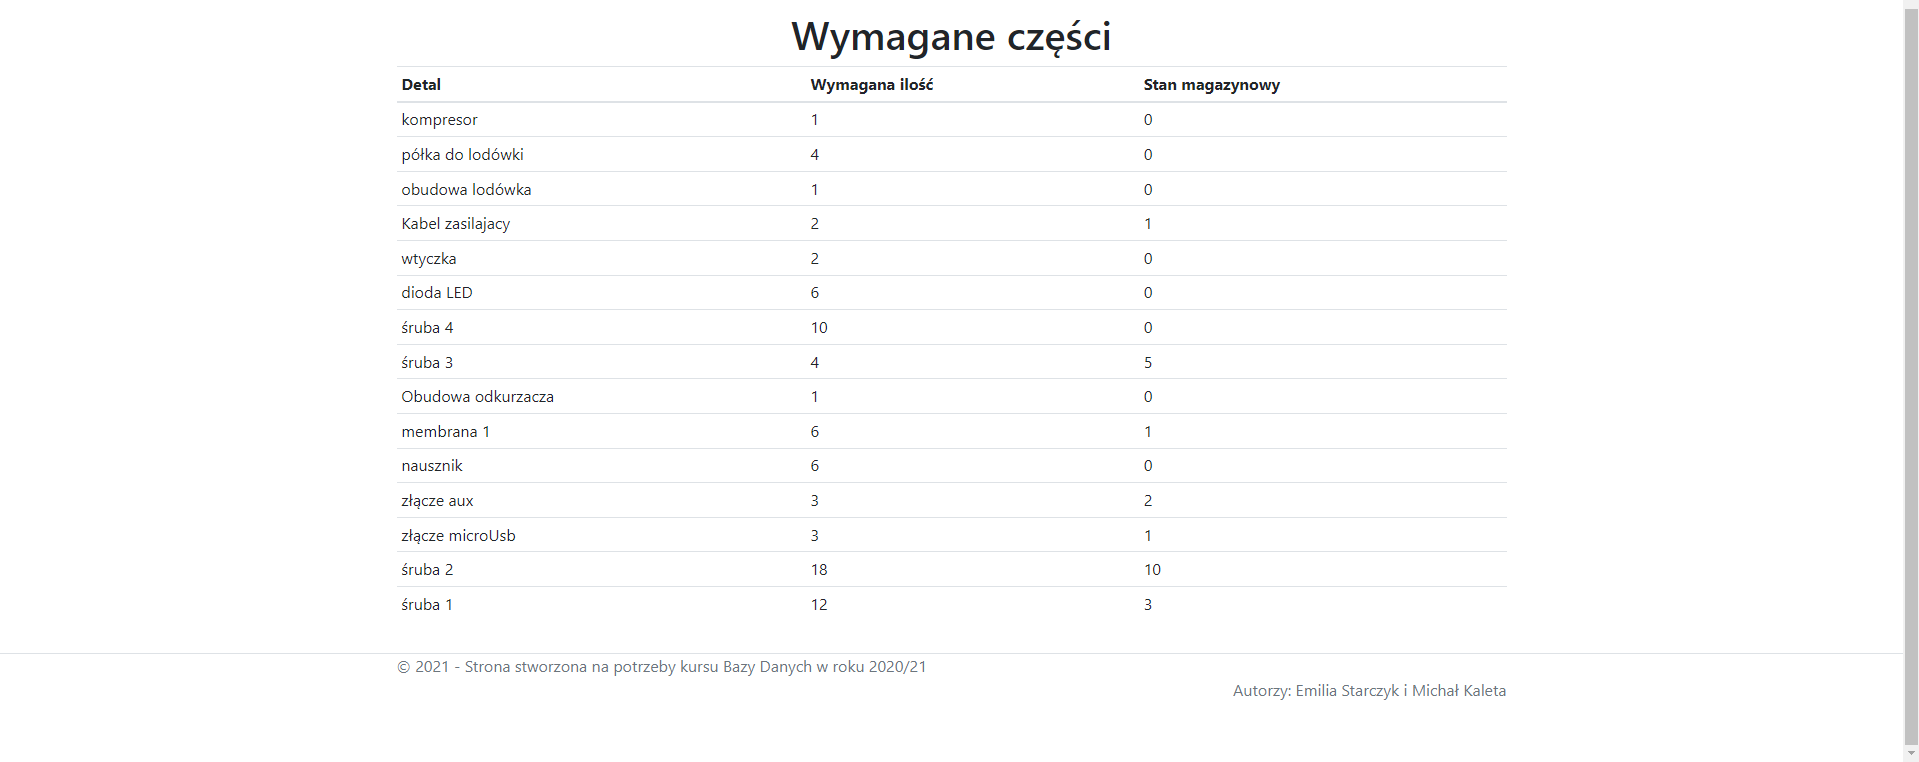
\includegraphics[width=0.6\textwidth]{Wyglad/szczegoly_zam2_admin.png}
            }}
         \captionof{figure}{Szczegóły pojedynczego zamówienia}
         W panelu ze szczegółami zamówienia administrator może podejrzeć ilości zamówionych produktów.
         Oprócz tego wyświetlana jest lista wszystkich wymaganych części do konkretnego zamówienia w
         zestawieniu z ilością dostępnych części na magazynie.
\end{itemize}

\subsubsection{Zamów części dodatkowe}
\begin{figure}[H]
   \centering
   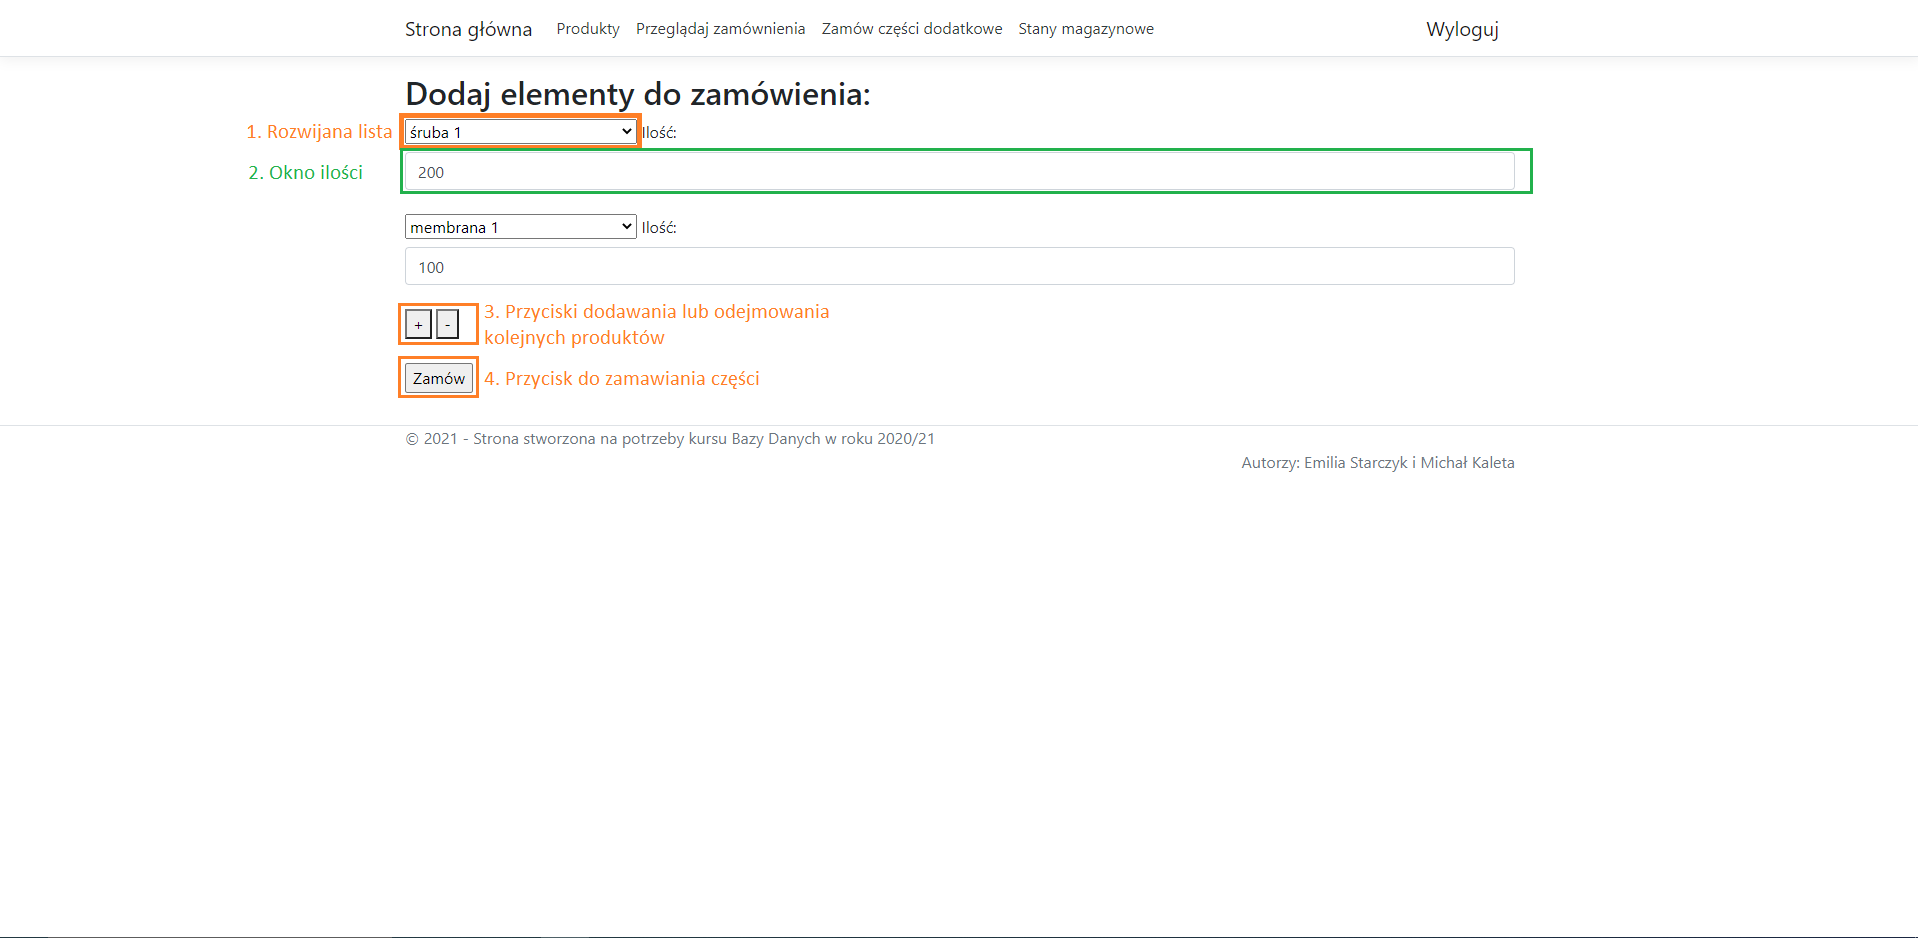
\includegraphics[width=0.99\textwidth,frame]{Wyglad/czesci_dodatkowe_admin.png}
   \caption{Widok strony pozwalającej na ręczne zamawianie części do magazynu}
\end{figure}
Panel ten składa się z kilku elementów:
\begin{enumerate}
   \item Rozwijana lista - lista wyboru części do zamówienia
   \item Okno ilości - pole pozwalające wpisać ilość produktu do zamówienia
   \item Przyciski dodawania lub odejmowania kolejnych części. Po wciśnięciu przycisku ``+''
         dodajemy kolejne pole dla kolejnej części. Po wciśnięciu przycisku ``-'' zmniejszamy ilość
         rozwijanych list z której wcześniej wybraliśmy produkt.
   \item Przycisk ``Zamów''. Po wciśnięciu przycisku produkty zostają zamówione do magazynu i
         następuje automatyczne przekierowanie na stronę ``Stany magazynowe''.
\end{enumerate}

\subsubsection{Stany magazynowy}
\begin{figure}[H]
   \centering
   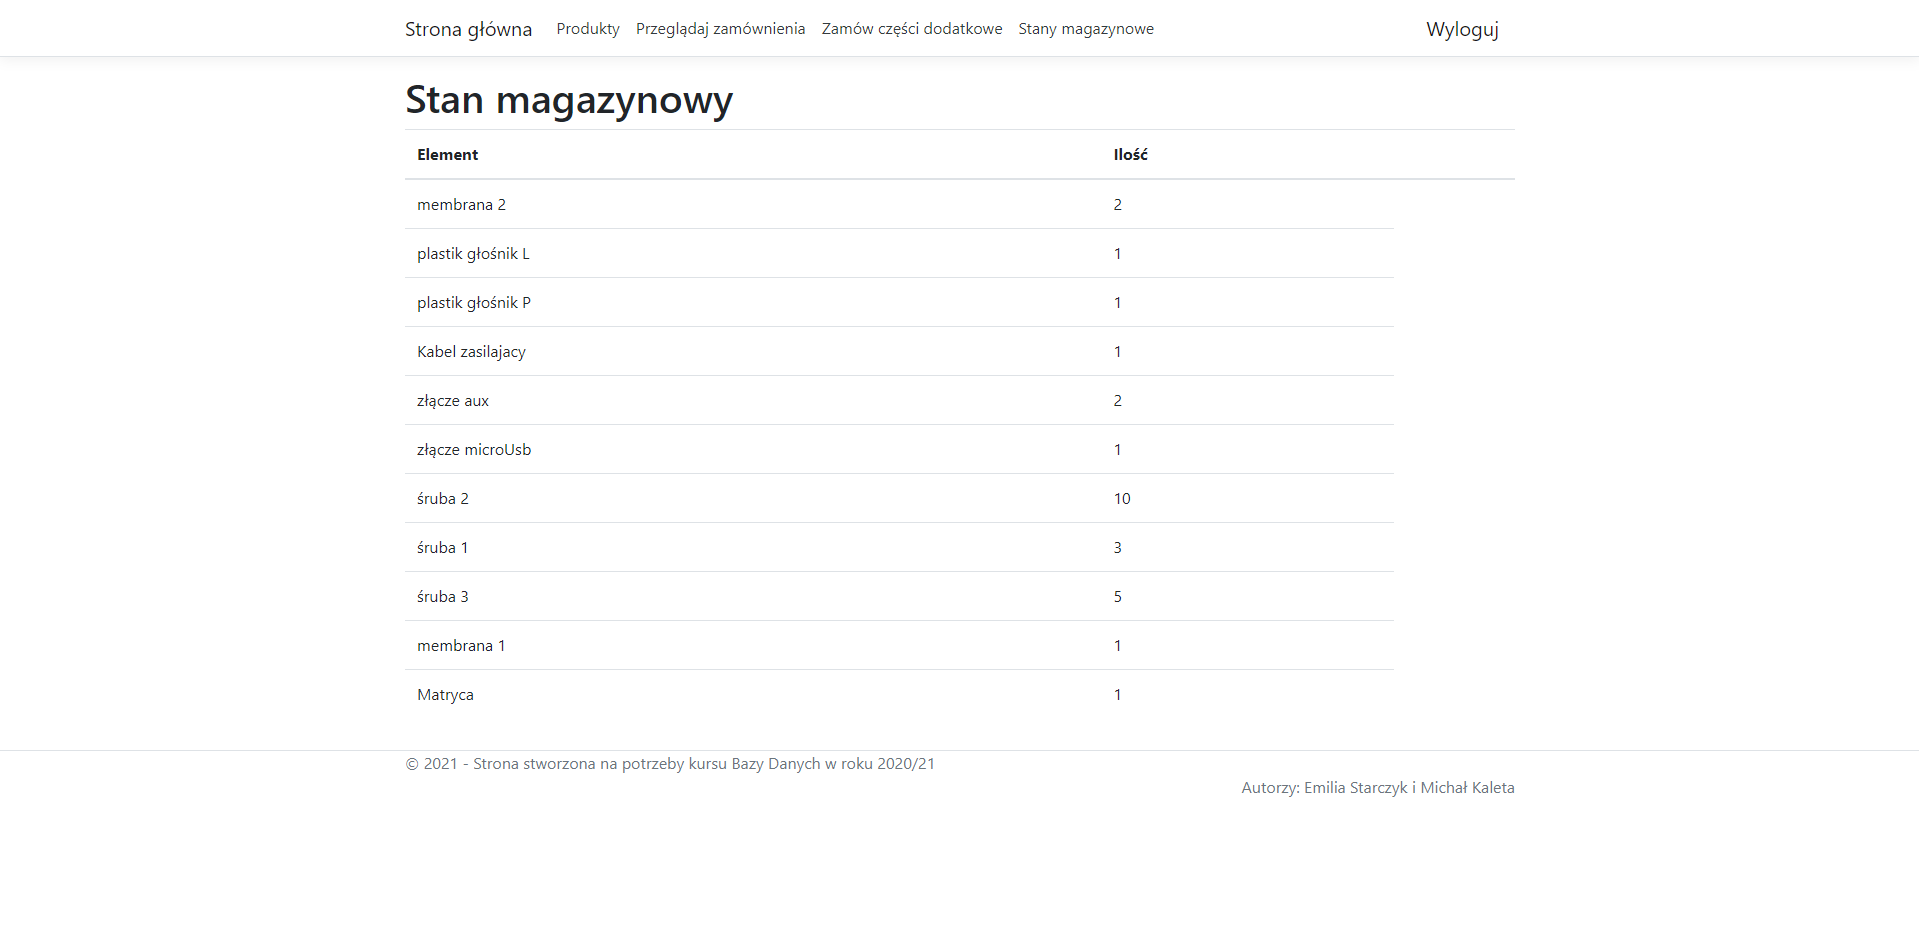
\includegraphics[width=0.99\textwidth,frame]{Wyglad/magazyn_admin.png}
   \caption{Widok strony przedstawiającej zawartość magazynu producenta przedmiotów}
\end{figure}

\subsubsection{Wyloguj}
\begin{figure}[H]
   \centering
   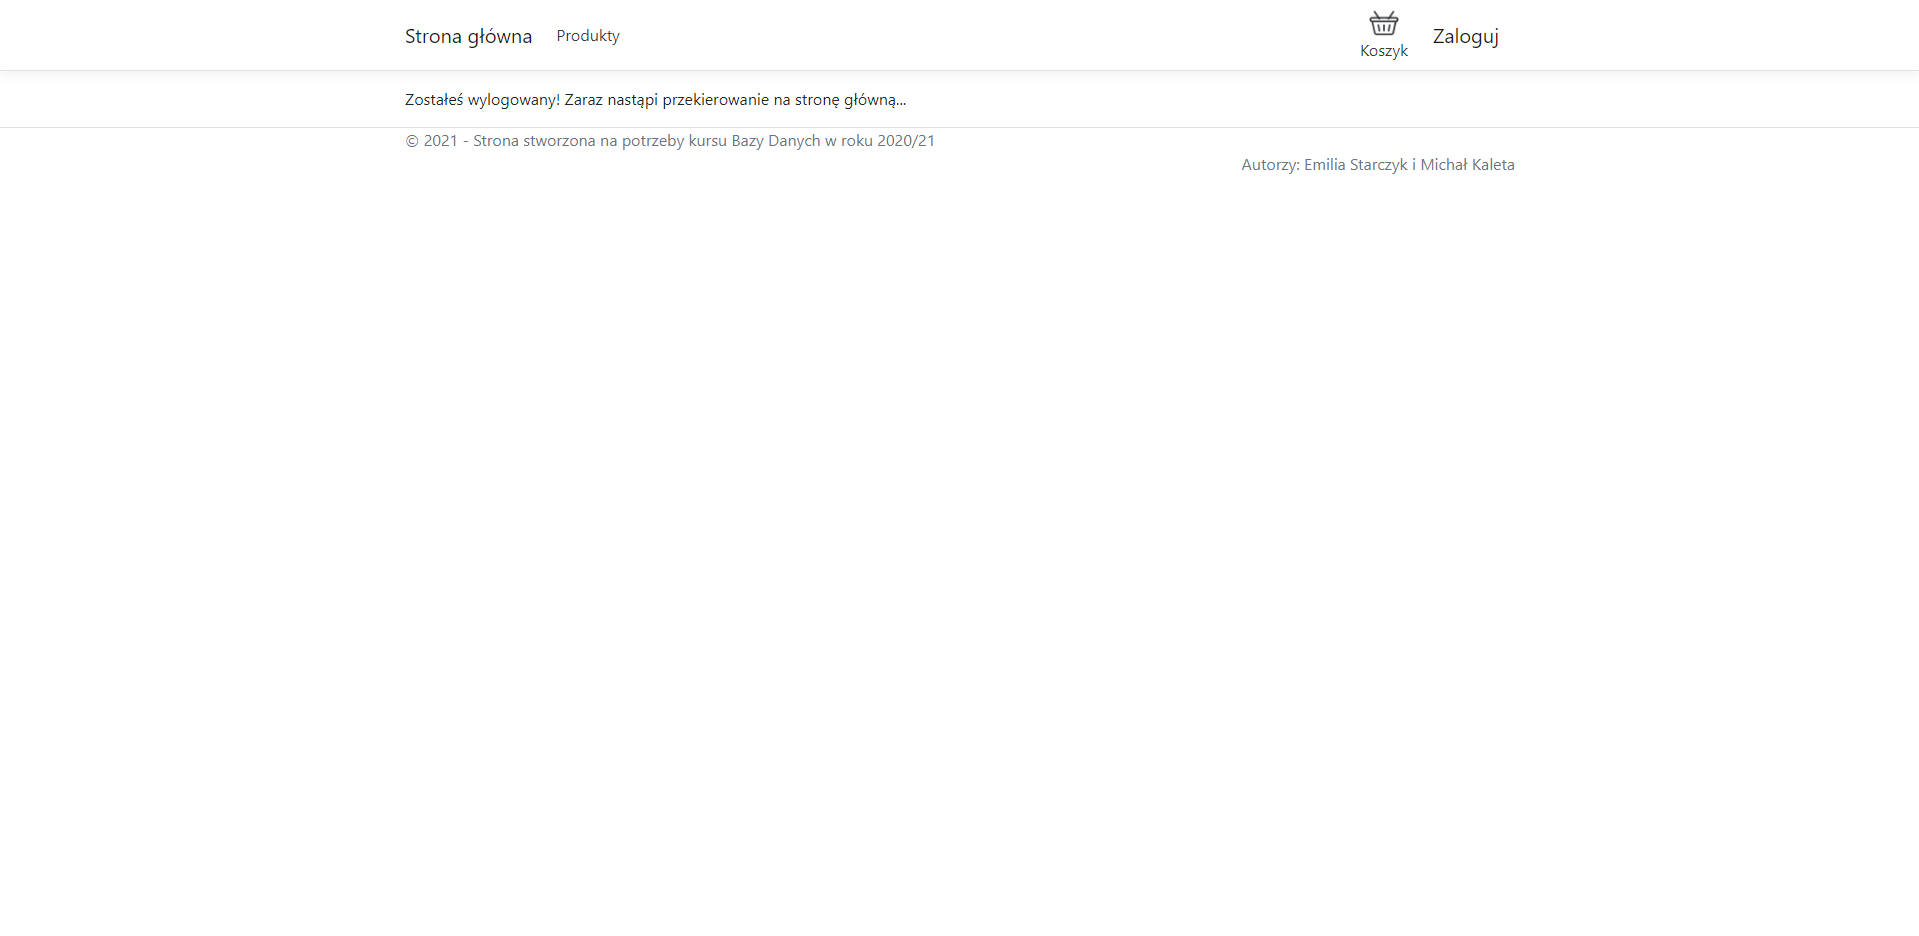
\includegraphics[width=0.99\textwidth,frame]{Wyglad/wylogowanie_admin.png}
   \caption{Widok strony po wciśnięciu przycisku ``Wyloguj'' w pasku nawigacyjnym}
\end{figure}

\end{document}